\documentclass[11pt]{article}
\usepackage[margin = 1in]{geometry}
\usepackage{amsmath}
\usepackage{amssymb}
\usepackage{amsthm} % for proof environment
\usepackage{enumitem}
\usepackage{graphicx}
\usepackage{indentfirst}
\usepackage{caption}
\usepackage{lscape}
\usepackage{multirow}
\usepackage{array}
\usepackage{subcaption} % caption the subfigures

\renewcommand{\labelenumii}{\alph*)}
\newcommand{\w}{\omega}
\newcommand{\p}{\prime}
\newcommand{\one}{\mathbf{1}}
\newcommand{\onep}{\mathbf{1}^\prime}
\newcommand{\lagr}{\mathcal{L}}
\newcommand{\inv}[1]{#1^{-1}}
\newcommand{\ev}{\mathbb{E}}
\renewcommand{\wp}{\omega^\prime}

\begin{document}
\begin{flushleft}
	Nick Hoffman \\
	Finance I, Spring 2020 A \\
	Assignment 1 \\
\end{flushleft}

\begin{enumerate}
	\item Useful facts
	\begin{enumerate}
		\item $ \ev[\w ^\p R ] = \w^\p \bar{R} $, where $\bar{R}$ is the $ N\times 1 $ vector of expected returns.
		\[\ev[\w^\p \bar{R}] = \ev\left[\sum_{i = 1}^{N}\tilde{R}_n \w_n\right] = \sum_{i = 1}^N \w_n \ev[\tilde{R}_n] = \w^\p \bar{R} \]
		
		\item $ \frac{\partial \ev[R^\p \w]}{\partial \w_n} = R_n $, or the entire vector $  \frac{\partial \ev[R^\p \w]}{\partial \w} = R $
		
		As in (a),
		\[\ev[\w^\p \bar{R}] =\sum_{i = 1}^N \w_n \ev[\tilde{R}_n]\]
		and thus
		\[\frac{\partial \ev[R^\p \w]}{\partial \w_n} = \ev[\tilde{R}_n] = \bar{R}\]
		and so in vector form,
		\[ \frac{\partial \ev[R^\p \w]}{\partial \w} = R\]
		
		\item $ V(R^\p \w) = cov(R^\p \w, R^\p \w) $ where $ V $ is the variance-covariance matrix of returns, with typical element $ \sigma_{i,j} = cov(\tilde{R}_i, \tilde{R}_j) $.
		
		By definition, 
		\begin{align*}
		cov(R^\p \w, R^\p \w) &= \ev\left[\sum_{i = 1}^N \w_n \tilde{R}_n \cdot \sum_{i = 1}^N \w_n \tilde{R}_n\right] - \ev\left[\sum_{i = 1}^N \w_n \tilde{R}_n\right]^2 \\
		&= \sum_{i = 1}^N \sum_{j = 1}^N \w_i \w_j \ev[R_i R_j] - \sum_{i = 1}^N \sum_{j = 1}^N \w_i \w_j \ev[R_i] \ev[R_j] \\
		&= \sum_{i = 1}^N \sum_{j = 1}^N \w_i\w_j cov(R_i, R_j) \\
		&= \w^\p V\w
		\end{align*}
		
		\item $ cov(R^\p \w, R_n) = \w^\p V e_n $, where $ e_n = [0, \dots, 0, 1, 0, \dots, 0]^\p $, with 1 in the $ n^{th} $ position.
		
		Using the same definition for the covariance as above, 
		\begin{align*}
		cov(R^\p \w, R_n) &= \ev[R^\p \w R_n] - \ev[R^\p \w]\ev[R_n] \\
		&= \sum_{i = 1}^N \w_i \big(\ev[R_i R_n] - \ev[R_i]\ev[R_n]\big) \\
		&= \sum_{i = 1}^N \w_i cov(R_i, R_n)
		\end{align*} 
		The final sum above is the $ n^{th} $ entry of the matrix $ \w^\p V $, and thus $ cov(R^\p \w, R_n) = \w^\p V e_n $
		
		\item $ \frac{\partial V(R^\p \w)}{\partial \w_n} = 2 cov(R^\p \w, R_n) $
		
		As in part (c), 
		\[V(R^\p \w) = \sum_{i = 1}^N \sum_{j = 1}^N \w_i \w_j cov(R_i, R_j)\]
		Thus,

		\[\frac{\partial V(R^\p \w)}{\partial \w_n} = 2 \sum_{i = 1}^N \w_i cov(R_i, R_n) = 2 cov(R^\p \w, R_n) \]
		where the final equality follows from (d).
	\end{enumerate}
	\item The portfolio problem with risky assets is 
	\begin{gather*}
	\min_\w \frac{1}{2}\w^\p V \w \\
	\text{s.t.} \\
	\w^\p \bar{R} \geq \mu \\
	\w^\p \one = 1
	\end{gather*}
	where $ \one $ is the $N$-vector with 1 in every element. The Lagrangean for this problem is
	\[\lagr = \frac{1}{2}\wp V \w + \lambda_1\big[\mu - \wp\bar{R}\big] + \lambda_2\big[1 - \wp \one\big]\]
	
	with first-order conditions
	\begin{align}
	V\w &= \lambda_1\bar{R} - \lambda_2\one \label{foc_1_1} \\
	\mu &= \wp \bar{R} \label{foc_1_2} \\
	\wp \one &= 1 \label{foc_1_3}
	\end{align}
	To begin, premultiply (\ref{foc_1_1}) by $ \inv{V} $, yielding
	\[\w = \lambda_1 \inv{V}\bar{R} + \lambda_2\inv{V}\one\]
	Now, define the following two efficient portfolios:
	\begin{align*}
	\w_R &= \frac{\inv{V}\bar{R}}{\one^\p \inv{V} \bar{R}} \\
	\w_1 &= \frac{\inv{V} \one}{\one^\p \inv{V} \one}
	\end{align*}
	Thus, the form for $ \w $ above can be transformed in the following way:
	\begin{align*}
	\w^* &= \lambda_1 \inv{V}\bar{R} + \lambda_2\inv{V}\one \\ 
	&= \lambda_1\left(\frac{\one^\p \inv{V}\bar{R}}{\one^\p \inv{V}\bar{R}}\right)\inv{V}\bar{R} + \lambda_2\left(\frac{\one^\p \inv{V}\one}{\one^\p \inv{V}\one}\right)\inv{V}\one \\
	&= \big(\lambda_1\one^\p \inv{V}\bar{R}\big)\w_R + \big(\lambda_2\one^\p \inv{V}\one\big)\w_1 \\
	&\equiv \alpha \w_R + (1 - \alpha)\w_1
	\end{align*}
	
	To show the final equality (i.e., that the weights on portfolios $ \w_R $ and $ w_1 $ sum to unity), we premultiply both sides by $ \one^\p $ and impose  (\ref{foc_1_3}):
	\[\onep \w^*= \big(\lambda_1\one^\p \inv{V}\bar{R}\big)\onep w_R + \big(\lambda_2\one^\p \inv{V}\one\big)\onep w_1 \]
	Because $ \w^* $, $ \w_R $, and $ \w_1 $ are portfolios, the above implies that 
	\[1 = \big(\lambda_1\one^\p \inv{V}\bar{R}\big) + \big(\lambda_2\one^\p \inv{V}\one\big)\]
	To solve for $\alpha$, we impose (\ref{foc_1_2}):
	\begin{align*}
	\w^{*\p}\bar{R} = \mu &\implies \alpha \w_R^\p \bar{R} + (1 - \alpha) \w_1^\p \bar{R} = \mu \\
	& \implies \alpha = \frac{\mu - \w_1^\p \bar{R}}{\w_R^\p \bar{R} - \w_1^\p \bar{R}}
	\end{align*}
	
	\item To find the Global Minimum Variance (GMV) portfolio, the problem is similar:
	\begin{gather*}
	\min_\w \frac{1}{2}\w^\p V \w \\
	\text{s.t.} \\
	\w^\p \one = 1
	\end{gather*}
	
	The Lagrangean for this problem is 
	\[\lagr = \frac{1}{2} \wp V \w + \lambda[1 - \wp \one ]\]
	From the first-order condition for $\omega$, we can use the same method as in question 2:
	\begin{align*}
	\w^* &= \lambda \inv{V} \one  \\
	&= \lambda\left(\frac{\one^\p \inv{V}\one}{\one^\p \inv{V}\one}\right)\inv{V}\one \\
	&= \big(\lambda \onep \inv{V}\one \big)\w_1
	\end{align*}
	Because $ \w $ and $ \w_1 $ are both portfolios, premultiplying the final line above by $ \onep $ shows that $ (\lambda \onep \inv{V}\one) = 1 $. Thus, $ \w_1 $ is the GMV portfolio
	
	\item With both risky assets and one risk-free asset, the problem becomes
	\begin{gather*}
	\min_\w \frac{1}{2}\w^\p V \w \\
	\text{s.t.} \\
	(1 - \w^\p \one)R_f + \w^\p \bar{R} \geq \mu
	\end{gather*}
	\begin{enumerate}
		\item The Lagrangian for this problem is as follows:
		\[\lagr = \frac{1}{2}\w^\p V \w + \lambda \big[\mu - (1 - \w^\p \one)R_f - \w^\p \bar{R}\big] \]
		with first-order conditions
		\begin{align}
		V\w + \lambda(\one R_f - \bar{R}) &= \mu \label{foc_4_1}\\
		(1 - \w^\p \one)R_f + \w^\p \bar{R} &\geq \mu \label{foc_4_2}
		\end{align}
		To begin, premultiply (\ref{foc_4_1}) by $ \inv{V} $ (assuming that $ V $ is invertible):

		\begin{equation}\label{step2_4}
		\w = \lambda \inv{V} \big(\bar{R} - \one R_f\big)
		\end{equation}
		
		Similarly, from (\ref{foc_4_2}), 
		\[\big(\bar{R} - \one R_f\big)\wp = \mu - R_f\]
		Thus, premultiplying (\ref{step2_4}) by $ (\bar{R} - \one R_f) $ gives
		\[\lambda\big(\bar{R} - \one R_f\big) \inv{V} \big(\bar{R} - \one R_f\big)\]
		and thus
		\[\lambda = \frac{\mu - R_f}{(\bar{R} - \one R_f\big) \inv{V} \big(\bar{R} - \one R_f )}\]
		Therefore, the optimal $ \w $ is given by 
		\[\w = \frac{\mu - R_f}{(\bar{R} - \one R_f\big) \inv{V} \big(\bar{R} - \one R_f )} \inv{V} \big(\bar{R} - \one R_f\big) \]
		
		\item To verify that the efficient frontier is linear in $ \sigma_p $, note that the variance of this portfolio is given by 
		\begin{align*}
		\wp V\w &= \frac{\mu - R_f}{(\bar{R} - \one R_f\big) \inv{V} \big(\bar{R} - \one R_f )} \big(\bar{R} - \one R_f\big)^\p \inv{V} V \frac{\mu - R_f}{(\bar{R} - \one R_f\big) \inv{V} \big(\bar{R} - \one R_f )} \inv{V} \big(\bar{R} - \one R_f\big) \\
		&= \frac{(\mu - R_f)^2}{\inv{V} \big(\bar{R} - \one R_f\big)}
		\end{align*}
		And thus the variance is 
		\[\sigma_p = \sqrt{\wp V \w} = \frac{|\mu - R_f}{\sqrt{\inv{V} \big(\bar{R} - \one R_f\big)}}\]
		Thus, solving for the return $ \mu_p $ gives
		\[\mu_p = R_f \pm \sigma_p \sqrt{\inv{V} \big(\bar{R} - \one R_f\big)}\]
		Thus, the portfolio return is linear in the variance, and thus the efficient frontier is linear. 
		
		\item The optimal Sharpe Ratio portfolio is the portfolio $ \w $ which solves
		\[\max_\w \frac{\wp\bar{R} - R_f}{\sqrt{\wp V \w}}\]
		The first-order condition for this problem is 
		\[\frac{d}{d\w} = -\frac{1}{2}(\wp \bar{R}) - R_f (\wp V \w)^{-\frac{3}{2}} V\w + \bar{R}(\wp V \w)^{-\frac{1}{2}} = 0 \]
		
		The portfolio solving this problem is 
		\[\w^* = \frac{\inv{V}\big(\bar{R} - \one R_f\big)}{\onep \inv{V} \big(\bar{R} - \one R_f\big)} \]
		
		This is the portfolio where, given $ N $ risky assets, the efficient frontier for the assets is tangent to the efficient frontier for the risky assets plus a risk free asset. Thus, this portfolio is also the efficient portfolio that includes only risky assets, when both risky and risk-free assets are available. 
	\end{enumerate}

	\item The excess returns, variances, standard deviations, and Sharpe ratios for twenty of the industries in the data are shown here:
	
	
	% Table created by stargazer v.5.2.2 by Marek Hlavac, Harvard University. E-mail: hlavac at fas.harvard.edu
	% Date and time: Mon, Jan 27, 2020 - 15:57:22
	\begin{table}[!htbp] \centering 
		\caption{Selected Industries, Full Sample} 
		\label{} 
		\begin{tabular}{@{\extracolsep{5pt}} lcccc} 
			\\[-1.8ex]\hline 
			\hline \\[-1.8ex] 
			Industry & Excess Return & V & $ \sigma $ & Sharpe \\ 
			\hline \\[-1.8ex] 
			Agric & $4.288$ & $5.477$ & $23.402$ & $14.051$ \\ 
			Autos & $3.679$ & $5.156$ & $22.706$ & $11.800$ \\ 
			Boxes & $6.114$ & $4.784$ & $21.873$ & $23.382$ \\ 
			Clths & $7.086$ & $4.965$ & $22.281$ & $27.312$ \\ 
			Cnstr & $5.058$ & $4.656$ & $21.577$ & $18.805$ \\ 
			Coal & $2.349$ & $7.407$ & $27.216$ & $4.958$ \\ 
			ElcEq & $7.167$ & $2.634$ & $16.229$ & $37.998$ \\ 
			Food & $7.965$ & $3.390$ & $18.412$ & $37.828$ \\ 
			Fun & $9.075$ & $2.985$ & $17.277$ & $46.735$ \\ 
			Guns & $8.408$ & $4.416$ & $21.014$ & $35.251$ \\ 
			Hardw & $5.550$ & $6.558$ & $25.609$ & $17.766$ \\ 
			Oil & $6.350$ & $3.813$ & $19.527$ & $27.397$ \\ 
			PerSv & $2.403$ & $5.429$ & $23.299$ & $6.023$ \\ 
			RlEst & $1.309$ & $3.987$ & $19.968$ & $1.548$ \\ 
			Smoke & $9.989$ & $6.126$ & $24.751$ & $36.319$ \\ 
			Softw & $1.129$ & $4.038$ & $20.095$ & $0.642$ \\ 
			Steel & $1.126$ & $4.152$ & $20.376$ & $0.619$ \\ 
			Txtls & $5.489$ & $3.670$ & $19.157$ & $23.431$ \\ 
			Util & $5.983$ & $7.262$ & $26.949$ & $18.492$ \\ 
			Whlsl & $6.587$ & $5.807$ & $24.098$ & $23.184$ \\ 
			\hline \\[-1.8ex] 
		\end{tabular} 
	\end{table} 
	
	\newpage
	\item Efficient frontiers
		\begin{figure}[!hbtp]
			\caption{Efficient Frontiers}
			\begin{subfigure}{.5\textwidth}
				\centering
				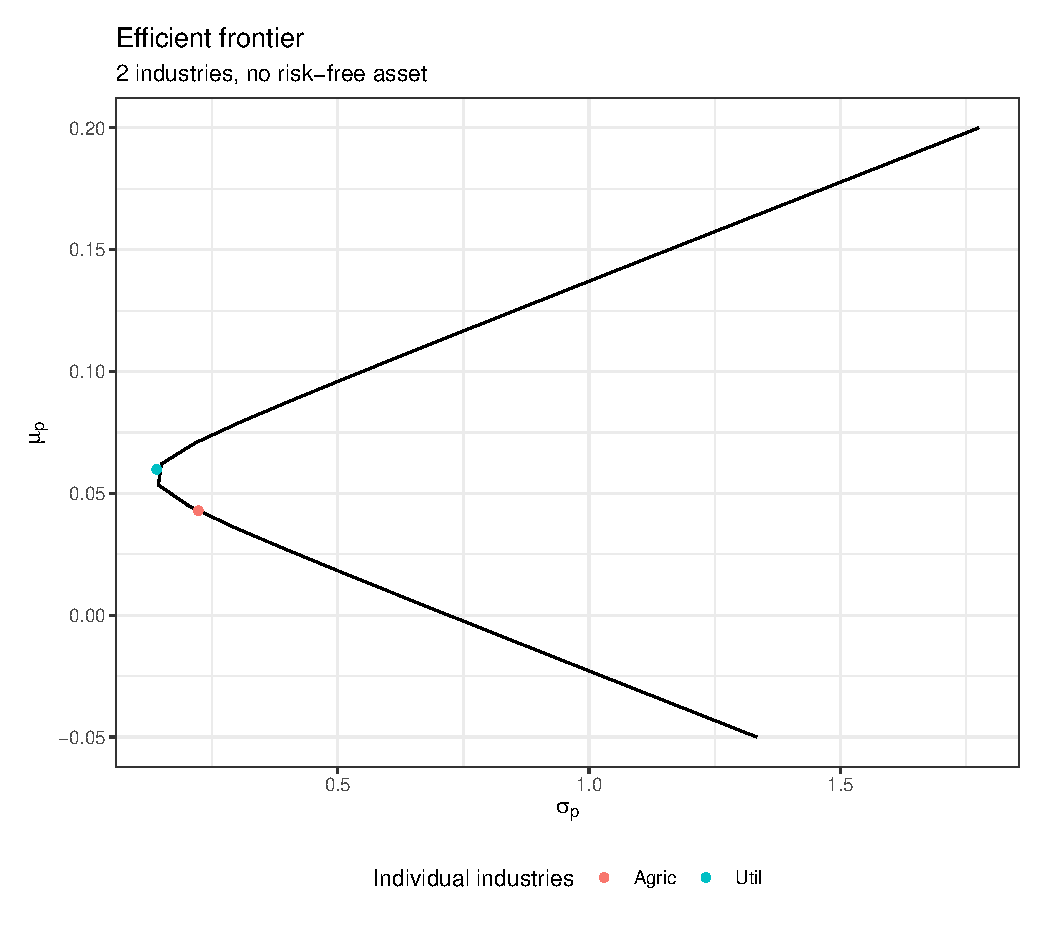
\includegraphics[width=.8\linewidth]{plot_6a.eps}
				\caption{Two-asset case}
				\label{fig1_a}
			\end{subfigure}%
			\begin{subfigure}{.5\textwidth}
				\centering
				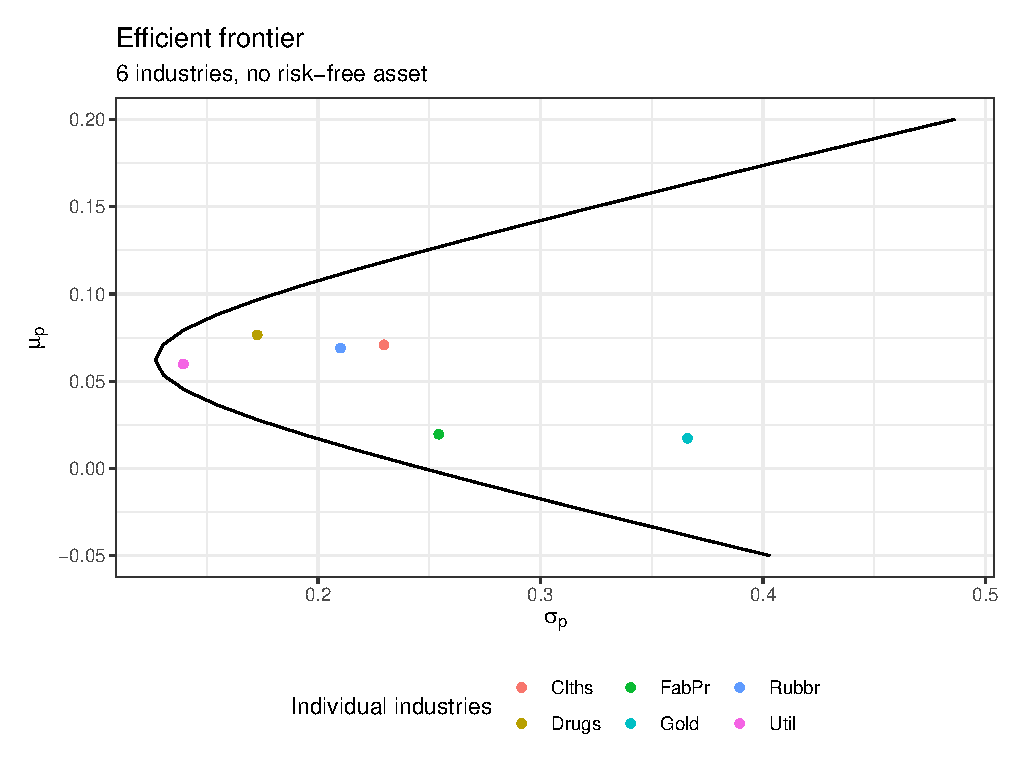
\includegraphics[width=.8\linewidth]{plot_6b}
				\caption{Six-asset case}
				\label{fig1_b}
			\end{subfigure}
			\label{fig1}
		\end{figure}
	
	\begin{figure}[!hbtp]
		\caption{Efficient Frontiers, with Risk-Free Rate of 1\%}
		\begin{subfigure}{.5\textwidth}
			\centering
			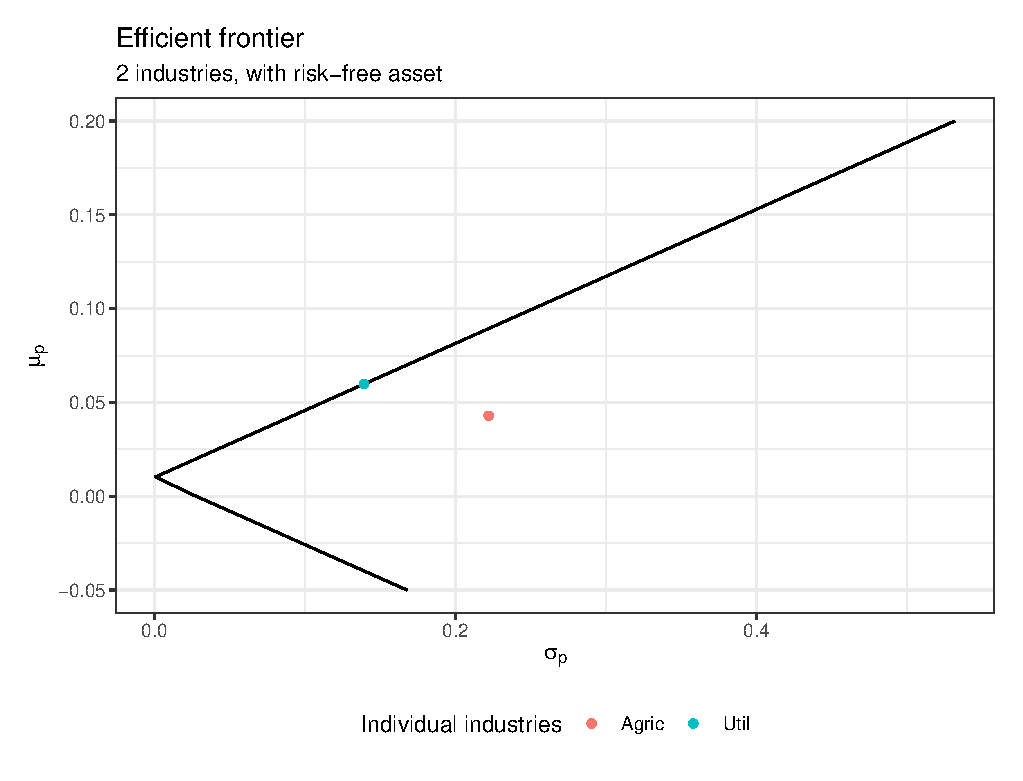
\includegraphics[width=.8\linewidth]{plot_6c.eps}
			\caption{Two-asset case}
			\label{fig2_a}
		\end{subfigure}%
		\begin{subfigure}{.5\textwidth}
			\centering
			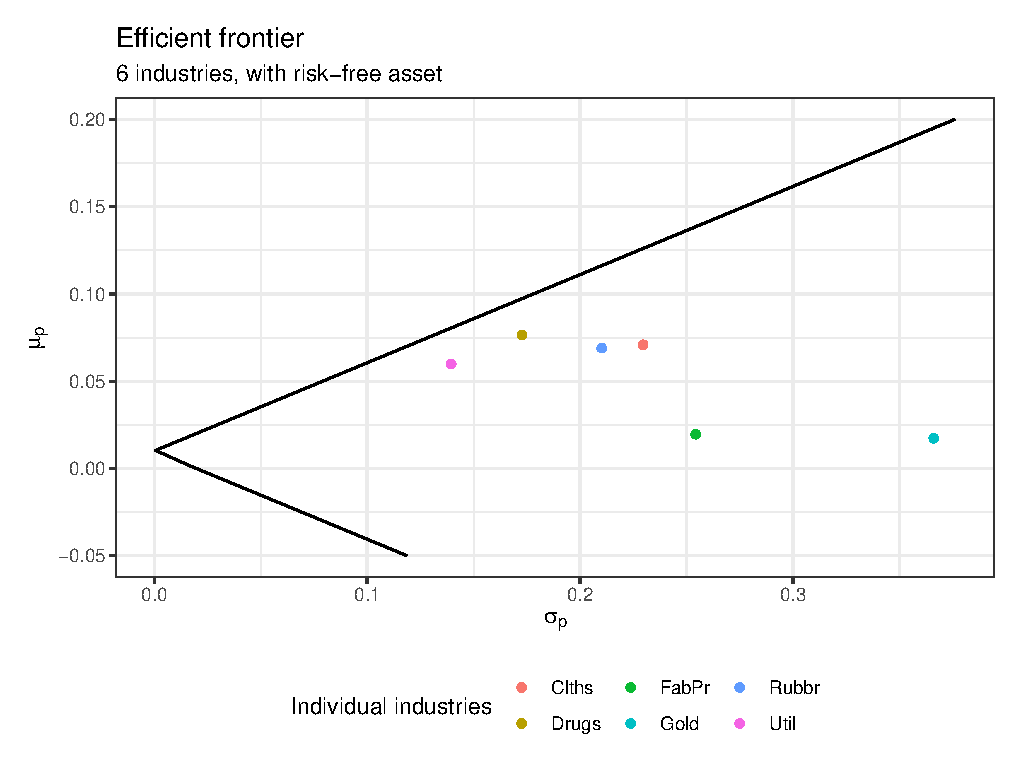
\includegraphics[width=.8\linewidth]{plot_6d}
			\caption{Six-asset case}
			\label{fig2_b}
		\end{subfigure}
		\label{fig2}
	\end{figure}
	
	\begin{enumerate}
		\item See Figure \ref{fig1_a}
		\item See Figure \ref{fig1_b}
		\item See Figure \ref{fig2}
		\newpage
		\item The above plots are generated by solving for $ \w^* $ as a function of $ \mu $, and plotting the efficient frontier in black at each value of $\mu$. 
		
		\begin{table}[!htbp] \centering 
			\caption{Example Weights} 
			\label{table_2} 
			\begin{tabular}{@{\extracolsep{5pt}} cccccccc} 
				\\[-1.8ex]\hline 
				\hline \\[-1.8ex] 
				$\mu_p$ & Gold & Clths & Rubbr & Drugs & Util & FabPr & $ \sigma_p $ \\ 
				\hline \\[-1.8ex] 
				$$-$0.050$ & $0.004$ & $$-$0.261$ & $0.032$ & $$-$0.050$ & $$-$0.463$ & $0.193$ & $0.088$ \\ 
				$$-$0.022$ & $0.002$ & $$-$0.140$ & $0.017$ & $$-$0.027$ & $$-$0.249$ & $0.103$ & $0.047$ \\ 
				$0.006$ & $0.0003$ & $$-$0.019$ & $0.002$ & $$-$0.004$ & $$-$0.034$ & $0.014$ & $0.007$ \\ 
				$0.033$ & $$-$0.001$ & $0.102$ & $$-$0.013$ & $0.019$ & $0.180$ & $$-$0.075$ & $0.034$ \\ 
				$0.061$ & $$-$0.003$ & $0.223$ & $$-$0.027$ & $0.042$ & $0.394$ & $$-$0.164$ & $0.075$ \\ 
				$0.089$ & $$-$0.005$ & $0.344$ & $$-$0.042$ & $0.065$ & $0.609$ & $$-$0.253$ & $0.116$ \\ 
				$0.117$ & $$-$0.006$ & $0.465$ & $$-$0.057$ & $0.088$ & $0.823$ & $$-$0.342$ & $0.157$ \\ 
				$0.144$ & $$-$0.008$ & $0.586$ & $$-$0.072$ & $0.111$ & $1.037$ & $$-$0.431$ & $0.198$ \\ 
				$0.172$ & $$-$0.010$ & $0.707$ & $$-$0.087$ & $0.134$ & $1.251$ & $$-$0.521$ & $0.239$ \\ 
				$0.200$ & $$-$0.011$ & $0.828$ & $$-$0.102$ & $0.157$ & $1.466$ & $$-$0.610$ & $0.279$ \\ 
				\hline \\[-1.8ex] 
			\end{tabular} 
		\end{table} 
		
		Table \ref{table_2} shows example weights $ \w^* $ (under the industry names) for the efficient frontier shown in Figure \ref{fig2_b}. $ \w^*_n < 0 $ indicates a short position in asset $ n $. Note that the weights do not sum to one; the remainder of the portfolio is held in the risk-free asset. 
		
	\end{enumerate}
	
	\item The following table and figure show the same exercise as in questions 5 and 6, but with the data limited to returns post-2000. 
	
	\begin{table}[!htbp] \centering 
		\caption{Returns Data, Post-2000} 
		\label{table_3} 
		\begin{tabular}{@{\extracolsep{5pt}} lcccc} 
			\\[-1.8ex]\hline 
			\hline \\[-1.8ex] 
			Industry & Excess Return & V & $\sigma_p$ & Sharpe \\ 
			\hline \\[-1.8ex] 
			Agric & $6.856$ & $5.477$ & $23.402$ & $25.022$ \\ 
			Autos & $1.330$ & $5.156$ & $22.706$ & $1.452$ \\ 
			Boxes & $8.918$ & $4.784$ & $21.873$ & $36.198$ \\ 
			Clths & $11.370$ & $4.965$ & $22.281$ & $46.542$ \\ 
			Cnstr & $8.701$ & $4.656$ & $21.577$ & $35.692$ \\ 
			Coal & $$-$2.351$ & $7.407$ & $27.216$ & $$-$12.311$ \\ 
			ElcEq & $4.997$ & $2.634$ & $16.229$ & $24.629$ \\ 
			Food & $7.941$ & $3.390$ & $18.412$ & $37.695$ \\ 
			Fun & $9.808$ & $2.985$ & $17.277$ & $50.979$ \\ 
			Guns & $15.340$ & $4.416$ & $21.014$ & $68.237$ \\ 
			Hardw & $1.721$ & $6.558$ & $25.609$ & $2.815$ \\ 
			Oil & $5.558$ & $3.813$ & $19.527$ & $23.344$ \\ 
			PerSv & $5.130$ & $5.429$ & $23.299$ & $17.728$ \\ 
			RlEst & $5.544$ & $3.987$ & $19.968$ & $22.755$ \\ 
			Smoke & $14.890$ & $6.126$ & $24.751$ & $56.118$ \\ 
			Softw & $3.779$ & $4.038$ & $20.095$ & $13.830$ \\ 
			Steel & $$-$0.392$ & $4.152$ & $20.376$ & $$-$6.834$ \\ 
			Txtls & $6.396$ & $3.670$ & $19.157$ & $28.166$ \\ 
			Util & $8.661$ & $7.262$ & $26.949$ & $28.429$ \\ 
			Whlsl & $7.201$ & $5.807$ & $24.098$ & $25.732$ \\ 
			\hline \\[-1.8ex] 
		\end{tabular} 
	\end{table} 
	
	\begin{figure}[!hbtp]
		\caption{Efficient Frontiers, Post-2000}
		\begin{subfigure}{.5\textwidth}
			\centering
			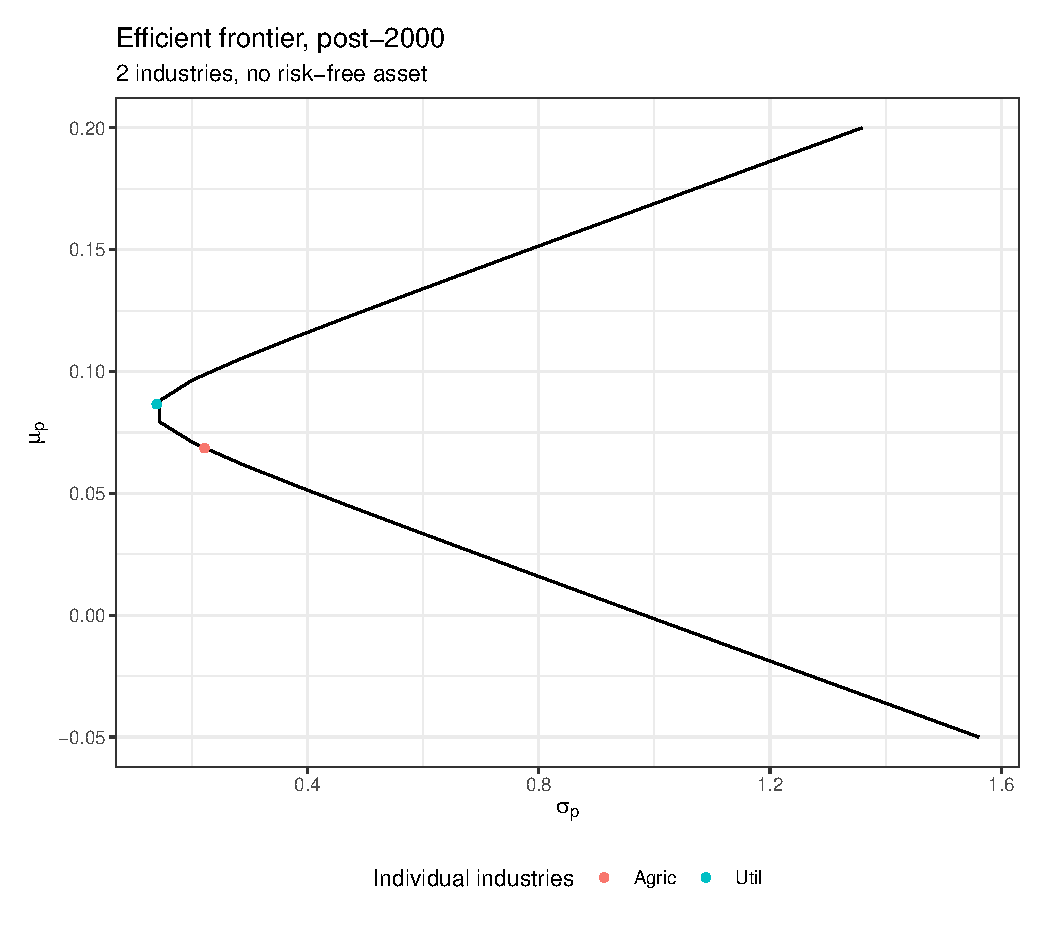
\includegraphics[width=.8\linewidth]{plot_7a.eps}
			\caption{Two-asset case}
			\label{fig3_a}
		\end{subfigure}%
		\begin{subfigure}{.5\textwidth}
			\centering
			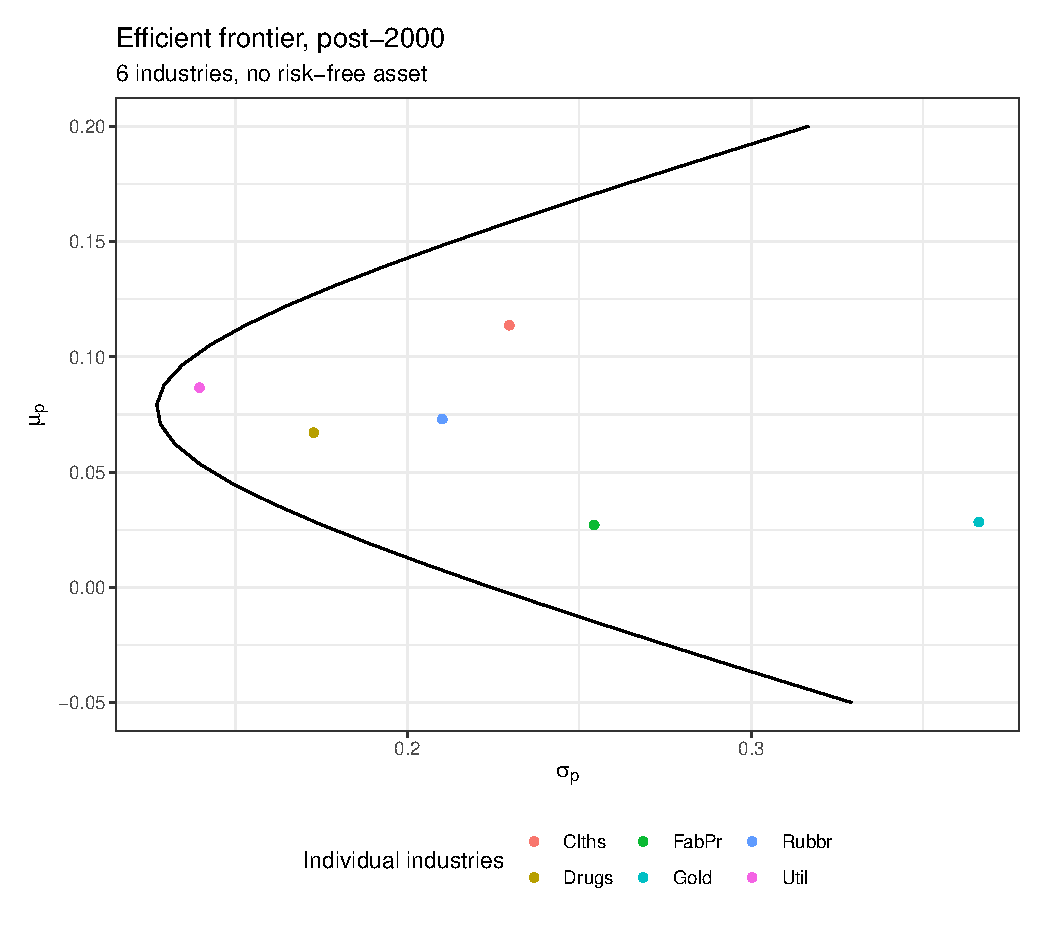
\includegraphics[width=.8\linewidth]{plot_7b.eps}
			\caption{Six-asset case}
			\label{fig3_b}
		\end{subfigure}
		\begin{subfigure}{.5\textwidth}
			\centering
			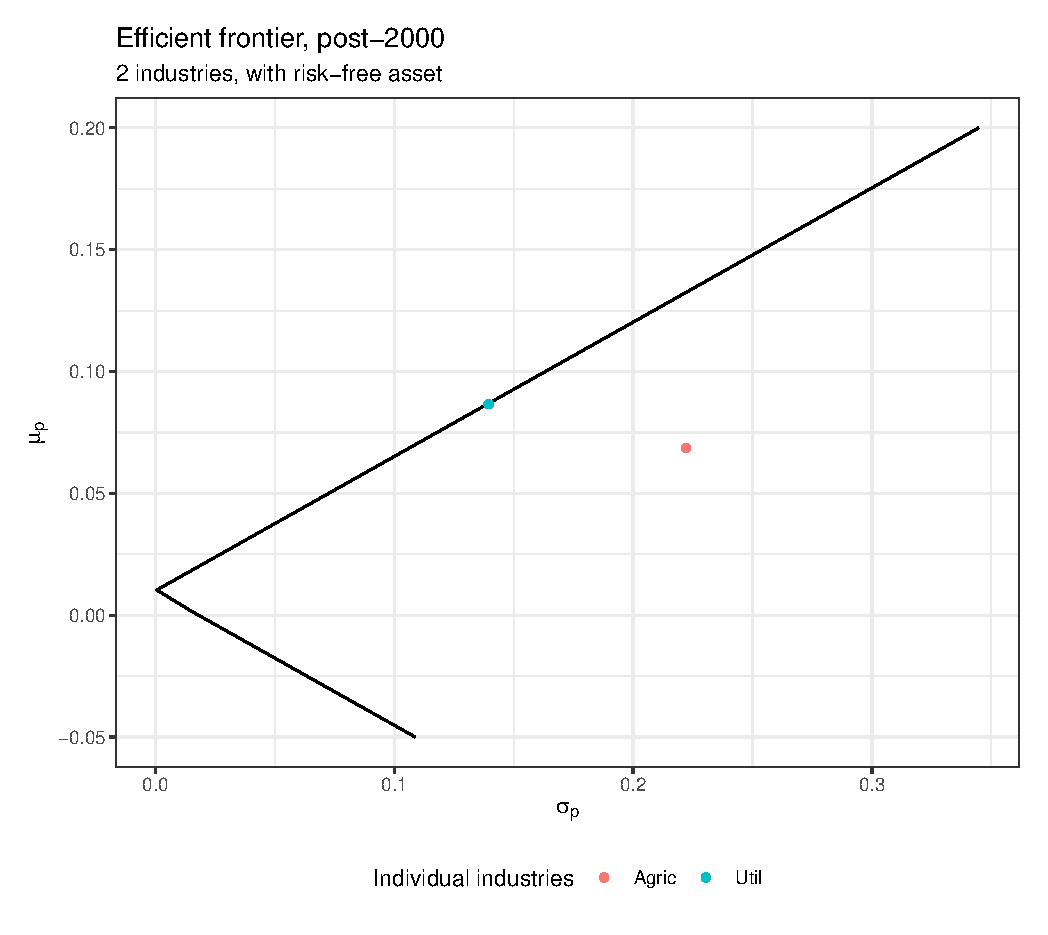
\includegraphics[width=.8\linewidth]{plot_7c.eps}
			\caption{Two-asset case}
			\label{fig3_c}
		\end{subfigure}%
		\begin{subfigure}{.5\textwidth}
			\centering
			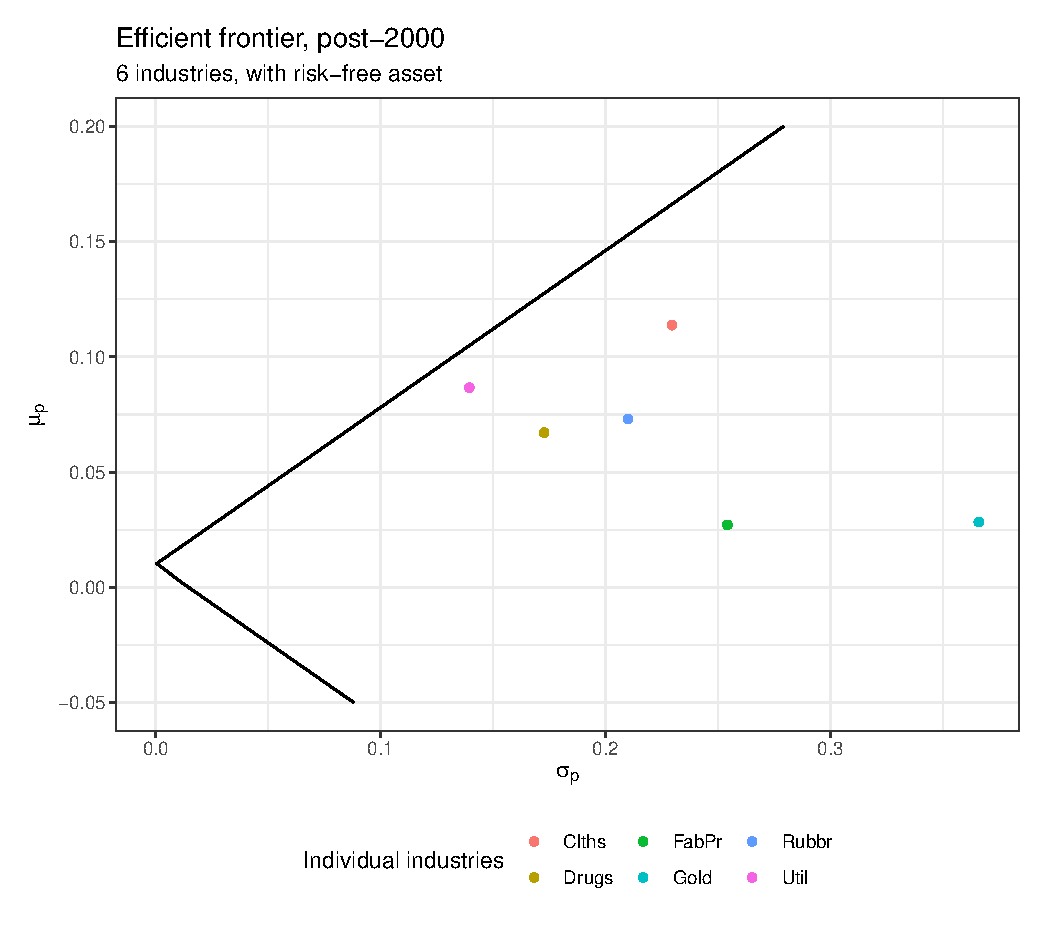
\includegraphics[width=.8\linewidth]{plot_7d.eps}
			\caption{Six-asset case}
			\label{fig3_d}
		\end{subfigure}
		\label{fig3}
	\end{figure}
	
	\newpage
	\item I constructed the Sharpe Ratio-maximal portfolio for all 1176 combinations of two assets in the data (excluding the ``market''). Of these, \textbf{589} have both portfolio weights nonnegative, and thus the probability that a portfolio of two of these industries does not include a short position is \textbf{50.1\%}. 
\end{enumerate}

\end{document}